\begin{table*}
\vspace{-0.2in}
\hspace{-0.6in}
\footnotesize
\begin{tabular}{|p{0.31in}|p{1in}|p{4in}|p{0.9in}|p{0.8in}|}
\hline
App Name & Example Input Video Frame & Description & Symbolic \phantom{000} Representation & Example Guidance \\
\hline
\phantom{000} \textbf{Pool}     & \raisebox{-0.9\totalheight}{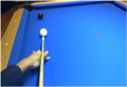
\psfig{file=FIGS/bigtable2/example-pool.png, width=0.97in}}
&
Helps a novice pool player aim correctly. Gives continuous visual feedback (left arrow, right arrow, or thumbs up) as the user turns his cue stick. Correct shot angle is calculated based on fractional aiming system~\cite{FractionalAiming}. Color, line, contour, and shape detection are used. The symbolic representation describes the positions of the balls, target pocket, and the top and bottom of cue stick.
&
\phantom{000} $<$Pocket, object ball, cue ball, cue top, cue bottom$>$ & \phantom{000} \raisebox{-0.85\totalheight}{
\psfig{file=FIGS/bigtable2/guidance-pool.png, width=0.8in}} \\
\hline
\phantom{000} \textbf{Ping-pong} & \raisebox{-0.9\totalheight}{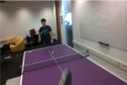
\psfig{file=FIGS/bigtable2/example-pingpong.png, width=0.97in}}
&
Tells novice to hit ball to the left or right, depending on which is more likely to beat opponent. Uses color, line and optical-flow based motion detection to detect ball, table, and opponent. The symbolic representation is a 3-tuple: in rally or not, opponent position, ball position. Whispers ``left'' or ``right'' or offers spatial audio guidance using~\cite{tang2014assistive}.

    Video URL: {\em \href{https://youtu.be/\_lp32sowyUA}{https://youtu.be/\_lp32sowyUA}}
&
\phantom{000} $<$InRally, ball position, opponent position$>$ & \phantom{000} Whispers ``Left!'' \\
\hline
\phantom{000} \textbf{Work-out} & \raisebox{-0.9\totalheight}{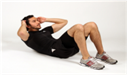
\psfig{file=FIGS/bigtable2/example-workout.png, width=0.97in}}
&
Guides correct user form in exercise actions like sit-ups and push-ups, and counts out repetitions. Uses Volumetric Template Matching~\cite{ke2007event} on a 10-15 frame video segment to classify the exercise.
%A poorly-performed repetition is classified as a distinct type of exercise (e.g. ``good pushup'' versus ``bad pushup'').
Uses smart phone on the floor for third-person viewpoint.
&
\phantom{000} $<$Action, count$>$ & \phantom{000} Says ``8 '' \\
\hline
\phantom{000} \textbf{Face}     & \raisebox{-0.9\totalheight}{
\psfig{file=FIGS/bigtable2/example-face.png, width=0.97in}}
&
Jogs your memory on a familiar face whose name you cannot recall. Detects and extracts a tightly-cropped image of each face, and then applies a state-of-art face recognizer using deep residual network~\cite{He2016}. Whispers the name of a person.
Can be used in combination with Expression~\cite{anam2014expression} to offer conversational hints.
&
\phantom{000} ASCII text of name & \phantom{000} Whispers ``Barack Obama'' \\
\hline
\phantom{000} \textbf{Lego} & \raisebox{-0.9\totalheight}{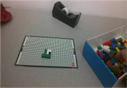
\psfig{file=FIGS/bigtable2/example-lego.png, width=0.97in}}
&
Guides a user in assembling 2D Lego models. Each video frame is analyzed in three steps: (i) finding the board using its distinctive color and black dot pattern; (ii) locating the Lego bricks on the board using edge and color detection; (iii) assigning brick color using weighted majority voting within each block. Color normalization is needed. The symbolic representation is a matrix representing color for each brick.

    Video URL: {\em \href{https://youtu.be/7L9U-n29abg}{https://youtu.be/7L9U-n29abg}}
&
\phantom{000} [[0, 2, 1, 1], \break [0, 2, 1, 6], \break [2, 2, 2, 2]] \break & \raisebox{-0.85\totalheight}{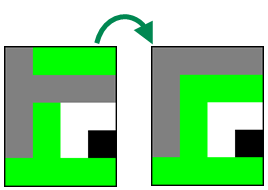
\psfig{file=FIGS/bigtable2/guidance-lego.png, width=0.8in}} Says ``Put a 1x3 green piece on top'' \\
\hline
\phantom{000} \textbf{Draw} & \raisebox{-0.9\totalheight}{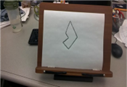
\psfig{file=FIGS/bigtable2/example-draw.png, width=0.97in}}
&
Helps a user to sketch better. Builds on third-party app~\cite{Iarussi2013} that was originally designed to take input sketches from pen-tablets and to output feedback on a desktop screen. Our implementation preserves the back-end logic. A new Glass-based front-end allows a user to use any drawing surface and instrument. Displays the error alignment in sketch on Glass.

    Video URL: {\em \href{https://youtu.be/nuQpPtVJC6o}{https://youtu.be/nuQpPtVJC6o}}
&
\raisebox{-0.85\totalheight}{
\psfig{file=FIGS/bigtable2/symbolic-draw.png, width=0.7in}} & \raisebox{-0.85\totalheight}{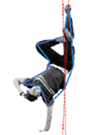
\psfig{file=FIGS/bigtable2/guidance-draw.png, width=0.8in}} \\
\hline
\phantom{000} \textbf{Sand-wich} & \raisebox{-0.9\totalheight}{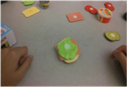
\psfig{file=FIGS/bigtable2/example-sandwich.png, width=0.97in}}
&
Helps a cooking novice prepare sandwiches according to a recipe. Since real food is perishable, we use a food toy with plastic ingredients. Object detection follows the state-of-art faster-RCNN deep neural net approach~\cite{ren2015faster}. Implementation is on top of Caffe~\cite{jia2014caffe} and Dlib~\cite{dlib09}. Transfer learning~\cite{Pan2010} helped us save time in labeling data and in training.

    Video URL: {\em \href{https://youtu.be/USakPP45WvM}{https://youtu.be/USakPP45WvM}}
&
\phantom{000} Object: \break ``E.g. Lettuce on top of ham and bread'' & \raisebox{-0.9\totalheight}{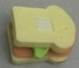
\psfig{file=FIGS/bigtable2/guidance-sandwich.jpg, width=0.7in}} Says ``Put a piece of bread on the lettuce'' \\
\hline

\end{tabular}
\caption{Prototype Wearable Cognitive Assistance Applications}
\label{fig:bg-apps-table}
\end{table*}